% Where this fit sits: stage 1 supplies the location of each parameter, stage 2
% (this talk) fits the population against published cohorts, and the deliverable
% is an ensemble of virtual populations.
%
%   compile:  pdflatex where_this_sits.tex
%
\documentclass[border=10pt]{standalone}
\usepackage{lmodern}
\usepackage{amsmath}
\usepackage{amssymb}
\usepackage{tikz}
\usetikzlibrary{arrows.meta,positioning,calc}
% Shared palette for the population-model figures.
%   ink      body / structure
%   popcol   the patient cloud and anything predicted from it
%   mechcol  the simulator and species-level quantities
%   msrcol   the measurement map (readout-level: gamma, kappa)
%   datacol  reported rows
\definecolor{ink}{HTML}{3A3A3A}
\definecolor{popcol}{HTML}{3B4AA6}
\definecolor{mechcol}{HTML}{2E7D5B}
\definecolor{msrcol}{HTML}{EB811B}
\definecolor{datacol}{HTML}{8C3B4A}

\newcommand{\Dset}{\mathcal{D}}

\begin{document}
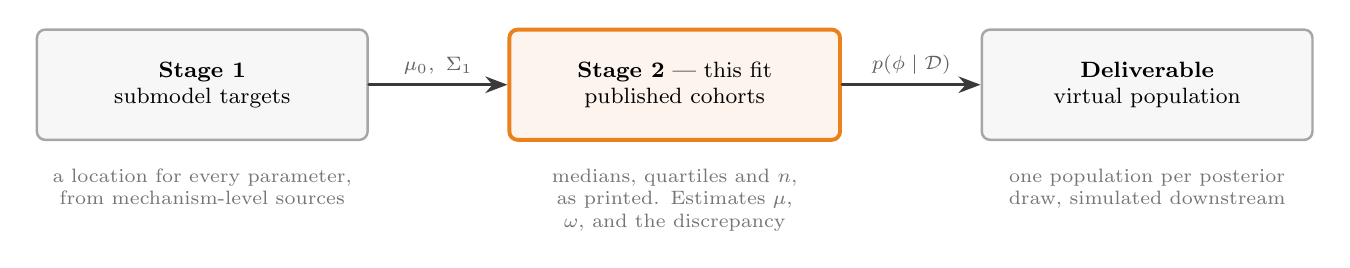
\begin{tikzpicture}[
  font=\sffamily, >=Stealth, line cap=round, line join=round,
  stg/.style={draw=ink!45, fill=ink!4, rounded corners=3pt, line width=0.9pt,
              minimum width=42mm, minimum height=14mm, inner sep=3pt,
              align=center, font=\footnotesize},
  here/.style={draw=msrcol, fill=msrcol!8, line width=1.4pt},
  sub/.style={font=\scriptsize, text=ink!70, align=center, anchor=north,
              text width=42mm},
  fl/.style={-{Stealth[length=2.8mm]}, ink, line width=1pt}]

\node[stg] (s1) at (0,0) {\textbf{Stage 1}\\ submodel targets};
\node[stg, here] (s2) at (6.0,0) {\textbf{Stage 2} --- this fit\\ published cohorts};
\node[stg] (s3) at (12.0,0) {\textbf{Deliverable}\\ virtual population};

\draw[fl] (s1) -- node[above, font=\scriptsize, ink!80] {$\mu_0,\ \Sigma_1$} (s2);
\draw[fl] (s2) -- node[above, font=\scriptsize, ink!80] {$p(\phi\mid\Dset)$} (s3);

\node[sub] at (0,-0.95)
  {a location for every parameter, from mechanism-level sources};
\node[sub] at (6.0,-0.95)
  {medians, quartiles and $n$, as printed. Estimates $\mu$, $\omega$, and the
   discrepancy};
\node[sub] at (12.0,-0.95)
  {one population per posterior draw, simulated downstream};

\end{tikzpicture}
\end{document}
